\documentclass[]{article}
\usepackage{lmodern}
\usepackage{amssymb,amsmath}
\usepackage{ifxetex,ifluatex}
\usepackage{fixltx2e} % provides \textsubscript
\ifnum 0\ifxetex 1\fi\ifluatex 1\fi=0 % if pdftex
  \usepackage[T1]{fontenc}
  \usepackage[utf8]{inputenc}
\else % if luatex or xelatex
  \ifxetex
    \usepackage{mathspec}
  \else
    \usepackage{fontspec}
  \fi
  \defaultfontfeatures{Ligatures=TeX,Scale=MatchLowercase}
\fi
% use upquote if available, for straight quotes in verbatim environments
\IfFileExists{upquote.sty}{\usepackage{upquote}}{}
% use microtype if available
\IfFileExists{microtype.sty}{%
\usepackage{microtype}
\UseMicrotypeSet[protrusion]{basicmath} % disable protrusion for tt fonts
}{}
\usepackage[margin=1in]{geometry}
\usepackage{hyperref}
\hypersetup{unicode=true,
            pdftitle={Analysis of electric vehicle usage patterns in New Zealand},
            pdfauthor={Rafferty Parker and Ben Anderson (University of Otago)},
            pdfborder={0 0 0},
            breaklinks=true}
\urlstyle{same}  % don't use monospace font for urls
\usepackage{longtable,booktabs}
\usepackage{graphicx,grffile}
\makeatletter
\def\maxwidth{\ifdim\Gin@nat@width>\linewidth\linewidth\else\Gin@nat@width\fi}
\def\maxheight{\ifdim\Gin@nat@height>\textheight\textheight\else\Gin@nat@height\fi}
\makeatother
% Scale images if necessary, so that they will not overflow the page
% margins by default, and it is still possible to overwrite the defaults
% using explicit options in \includegraphics[width, height, ...]{}
\setkeys{Gin}{width=\maxwidth,height=\maxheight,keepaspectratio}
\IfFileExists{parskip.sty}{%
\usepackage{parskip}
}{% else
\setlength{\parindent}{0pt}
\setlength{\parskip}{6pt plus 2pt minus 1pt}
}
\setlength{\emergencystretch}{3em}  % prevent overfull lines
\providecommand{\tightlist}{%
  \setlength{\itemsep}{0pt}\setlength{\parskip}{0pt}}
\setcounter{secnumdepth}{5}
% Redefines (sub)paragraphs to behave more like sections
\ifx\paragraph\undefined\else
\let\oldparagraph\paragraph
\renewcommand{\paragraph}[1]{\oldparagraph{#1}\mbox{}}
\fi
\ifx\subparagraph\undefined\else
\let\oldsubparagraph\subparagraph
\renewcommand{\subparagraph}[1]{\oldsubparagraph{#1}\mbox{}}
\fi

%%% Use protect on footnotes to avoid problems with footnotes in titles
\let\rmarkdownfootnote\footnote%
\def\footnote{\protect\rmarkdownfootnote}

%%% Change title format to be more compact
\usepackage{titling}

% Create subtitle command for use in maketitle
\newcommand{\subtitle}[1]{
  \posttitle{
    \begin{center}\large#1\end{center}
    }
}

\setlength{\droptitle}{-2em}

  \title{Analysis of electric vehicle usage patterns in New Zealand}
    \pretitle{\vspace{\droptitle}\centering\huge}
  \posttitle{\par}
  \subtitle{Summary Statistical Report}
  \author{Rafferty Parker and Ben Anderson (University of Otago)}
    \preauthor{\centering\large\emph}
  \postauthor{\par}
      \predate{\centering\large\emph}
  \postdate{\par}
    \date{Last run at: 2019-02-04 15:23:59}

\usepackage{booktabs}
\usepackage{longtable}
\usepackage{array}
\usepackage{multirow}
\usepackage{wrapfig}
\usepackage{float}
\usepackage{colortbl}
\usepackage{pdflscape}
\usepackage{tabu}
\usepackage{threeparttable}
\usepackage{threeparttablex}
\usepackage[normalem]{ulem}
\usepackage{makecell}
\usepackage{xcolor}

\begin{document}
\maketitle

{
\setcounter{tocdepth}{2}
\tableofcontents
}
\section{Note}\label{note}

Based on and inspired by the
\href{https://assets.publishing.service.gov.uk/government/uploads/system/uploads/attachment_data/file/764270/electric-chargepoint-analysis-2017-domestics.pdf}{UK
DoT statistical report 2018}.

This is a summary report. A discussion into the background around the
effects of EV charging in New Zealand, as well as detailed information
on data limitations and data cleaning procedure is given in the full
report.

\section{Data information}\label{data}

\subsection{Background}\label{background}

The data consisted of 1291881 data points (of which 790391 were charging
(power demand \textgreater{} 0)) from 50 vehicles over 8 months (April
2018 - January 2019) derived from FlipTheFleet's
\href{https://flipthefleet.org/ev-black-box/}{blackbox recorder}. The
recorder provided measurements at 1 minute frequency of charging
behaviour and battery charge state.

Due to privacy considerations, the data is not publically available.

\subsection{Definitions:}\label{definitions}

The capacity of most domestic charging is between 1.8kW to 7kW, whereas
charging power above 7kW is available at purpose-built charging
stations{[}@concept2018{]}. Each charging event was therefore seperated
into ``Fast'' (\textgreater{} = 7kW) and ``Standard'' (below 7kW).

A charging event was defined as a continuous sequence of 1 minute
observations per vehicle when \textgreater{} 0 kW of demand was
observed.

\subsection{Cleaning and Preparation}\label{cleaning-and-preparation}

\emph{Perhaps for the summary report this entire subsection could be
removed?} There were 6 vehicles within the provided data that had no
recorded charging occur. These were immediately discarded.

Some instances of charging power greater than 120kW were recorded. These
were considered anomolies and discarded, as these exceed the capacity of
the highest charging stations available in New Zealand{[}concept2018{]}.

Instances of battery state of charge being greater than 100\% or less
than 0\% were also discarded.

Standard charge durations of less than 8 minutes were frequently
encountered near the end of a longer charging cycle, where the state of
charge had reached it's maximum. These were assumed to be minor
`top-ups', and were discarded. In addition, slow charging events greater
than 100 hours were discarded, as were fast charge durations greater
than 14 hours. These were presumed anomolies as they exceed the battery
capacity of electric vehicles commonly encountered in New Zealand.

For more detailed information on the data cleaning process refer to the
main report.

\section{Key Findings:}\label{key-findings}

\begin{itemize}
\tightlist
\item
  \emph{Power supplied}: The median power supplied during a standard
  charging was 1.78 kW. The mean was slightly higher at 2.12 kW. Fast
  charging observations had a higher median of 30.84 kW (mean = 30.68);
\item
  \emph{Charging duration}: Charging durations tended to fall into one
  of two groups - longer `overnight' charges with a median of XX hours
  and shorter events during the day both at standard and fast charge
  rates with a median duration of XX hours.
\item
  \emph{Time of Day}: charging events were more frequent at specific
  times of the day and day of the week with more evening and over-night
  charging during weekdays and more day-time charging at weekends. The
  power demand also varied according to time of day and day of the week.
\end{itemize}

\section{Observed demand}\label{observed-demand}

Figure \ref{fig:obsPower} shows the distribution of observed charging kW
demand by inferred charge type. This plot shows that fast charges are
relatively rare in the dataset whilst standard charges are much more
common, and are concentrated around 1.8kW, 3kW and 6kW.

\begin{verbatim}
## `stat_bin()` using `bins = 30`. Pick better value with `binwidth`.
\end{verbatim}

\begin{figure}
\centering
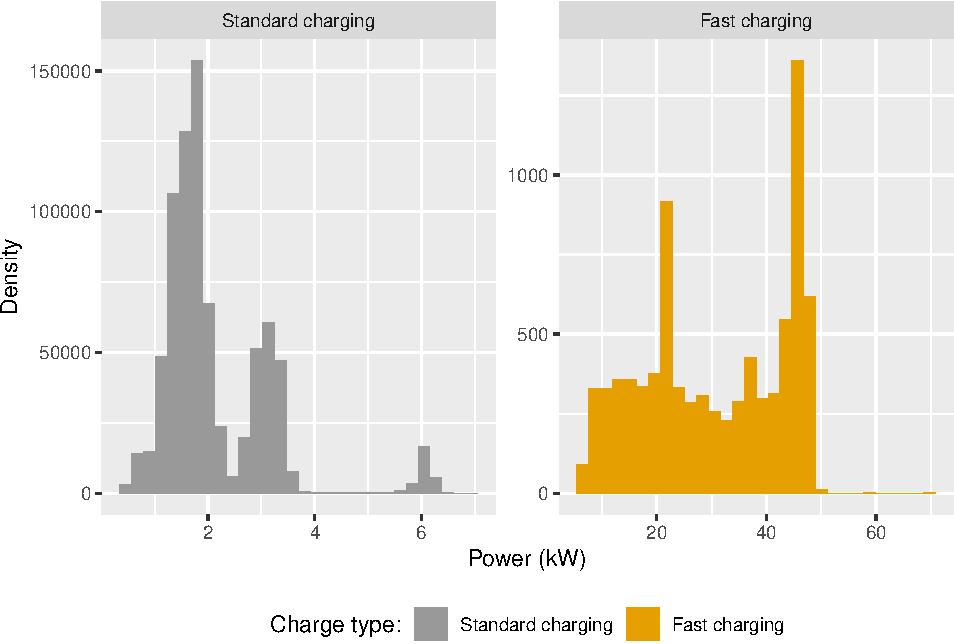
\includegraphics{EVBB_SummaryReport_files/figure-latex/obsPower-1.pdf}
\caption{\label{fig:obsPower}Observed power demand distribution by charge
type}
\end{figure}

75\% of standard charging observations were 1.47 kW or more but the
figure was 20.28 kW or more for fast charging

\section{Daily demand}\label{daily-demand}

\begin{figure}
\centering
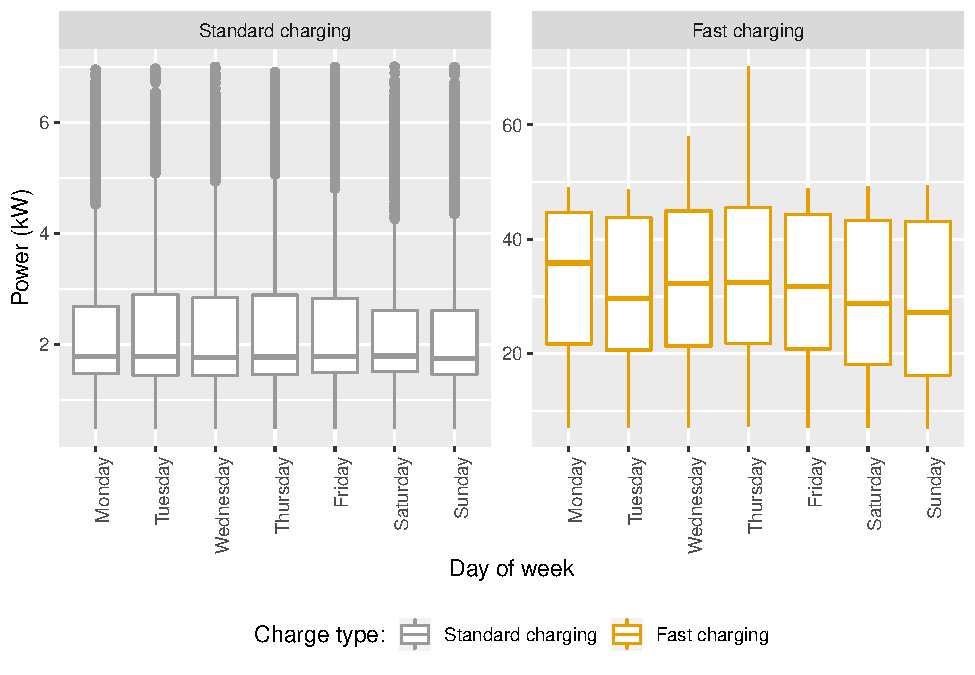
\includegraphics{EVBB_SummaryReport_files/figure-latex/dailyPower-1.pdf}
\caption{\label{fig:dailyPower}Observed power demand distribution by day of
the week and charge type}
\end{figure}

Figure \ref{fig:dailyPower} shows the distribution of observed charging
kW demand by day of the week. We can see that fast charging varies in
demand but standard charging is relatively constant across days.

\section{Charging duration}\label{duration}

Figure \ref{fig:durationHist} shows the overall distribution of charging
sequences. As would be expected, fast charging events tend to have a
much shorted duration than standard charging.

\begin{table}[t]

\caption{\label{tab:durationDescTableReduced}Duration (minutes) of charge sequences by charge type}
\centering
\begin{tabular}{l|r|r|r|r|r}
\hline
chargeType & N & mean & median & min & max\\
\hline
Standard charging & 2860 & 244.01 & 208.65 & 8.02 & 1616.72\\
\hline
Fast charging & 277 & 17.74 & 15.50 & 8.05 & 80.27\\
\hline
\end{tabular}
\end{table}

\begin{figure}
\centering
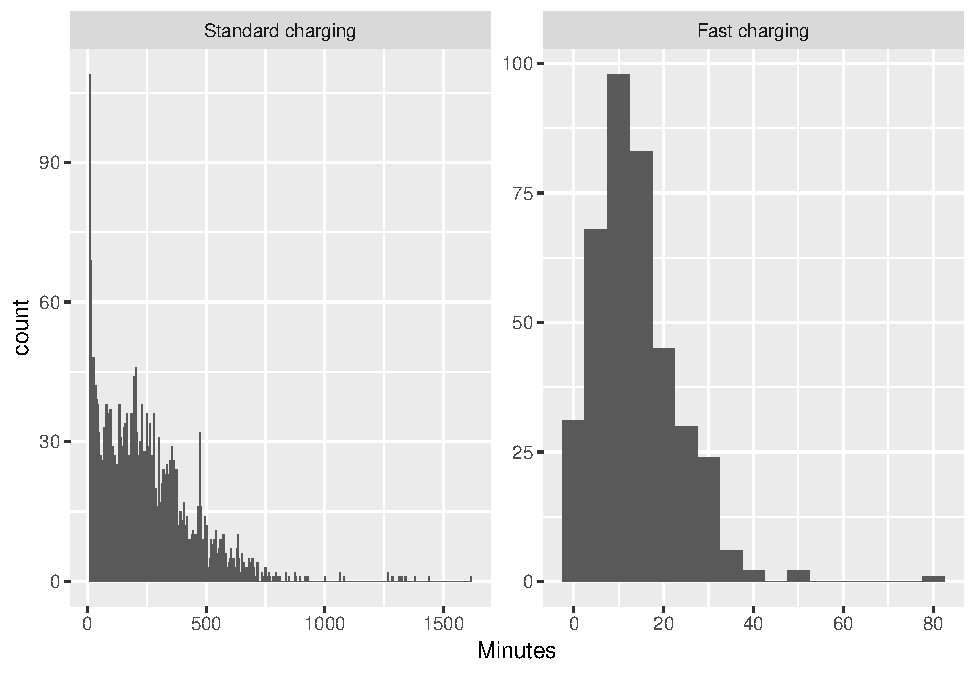
\includegraphics{EVBB_SummaryReport_files/figure-latex/durationHist-1.pdf}
\caption{\label{fig:durationHist}Duration of charging sequences}
\end{figure}

\begin{figure}
\centering
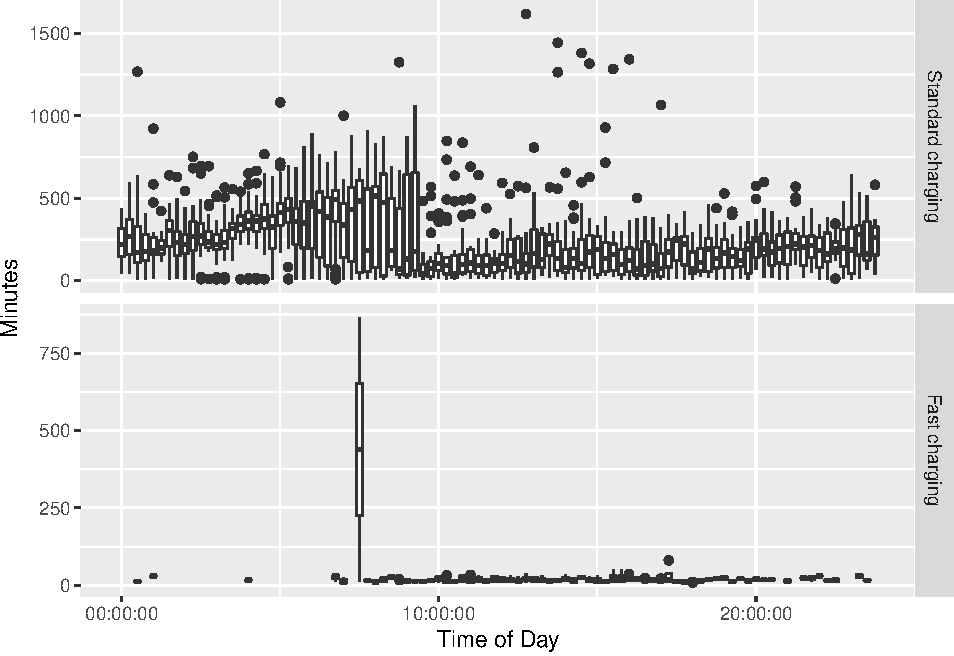
\includegraphics{EVBB_SummaryReport_files/figure-latex/durationTimeBox-1.pdf}
\caption{\label{fig:durationTimeBox}Duration by time of charging start for
sequences \textgreater{} 8 minutes}
\end{figure}

\begin{figure}
\centering
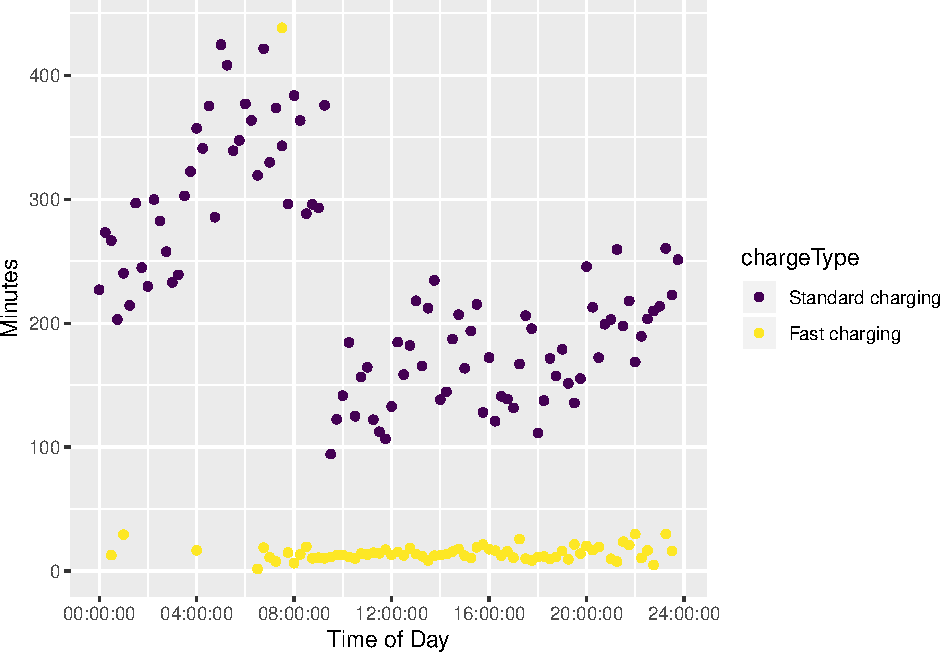
\includegraphics{EVBB_SummaryReport_files/figure-latex/durationTimeMean-1.pdf}
\caption{\label{fig:durationTimeMean}Mean duration (within quarter hours) by
time of charging start for sequences \textgreater{} 8 minutes}
\end{figure}

\begin{table}[t]

\caption{\label{tab:meanDurationTable}Mean duration of charge events by charge type}
\centering
\begin{tabular}{l|r|r|r|r|r}
\hline
chargeType & N & mean & median & min & max\\
\hline
Standard charging & 2860 & 244.00682 & 208.65 & 8.016667 & 1616.71667\\
\hline
Fast charging & 277 & 17.73694 & 15.50 & 8.050000 & 80.26667\\
\hline
\end{tabular}
\end{table}

\section{Time of charging}\label{time-of-charging}

\begin{figure}
\centering
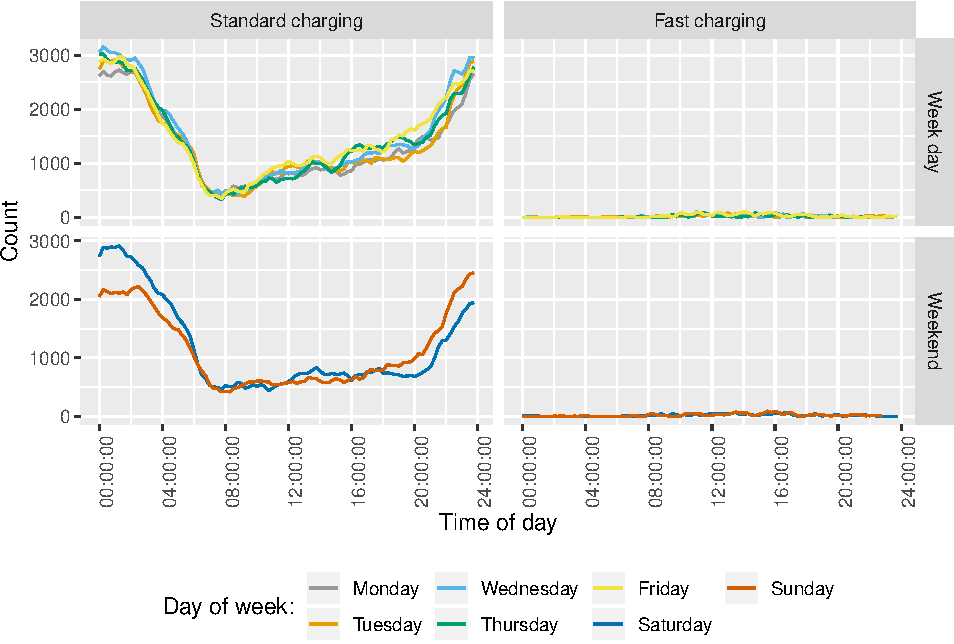
\includegraphics{EVBB_SummaryReport_files/figure-latex/chargeTime-1.pdf}
\caption{\label{fig:chargeTime}Count of observed charging events by type,
day of week and time}
\end{figure}

Figure \ref{fig:chargeTime} shows the distribution of observed charging
by time of day and day of the week. Aggregating counts in this way
emphasises the times at which charging most commonly occurs and we can
see\ldots{}

Fig: profile of median charging demand by time of day and day of the
week faceted by at home vs not at home

Charging demand varies somewhat by time of day and day of the week.
Weekdays show \ldots{} whilst weekends show. Saturdays and Sundays vary
with\ldots{}

\begin{figure}
\centering
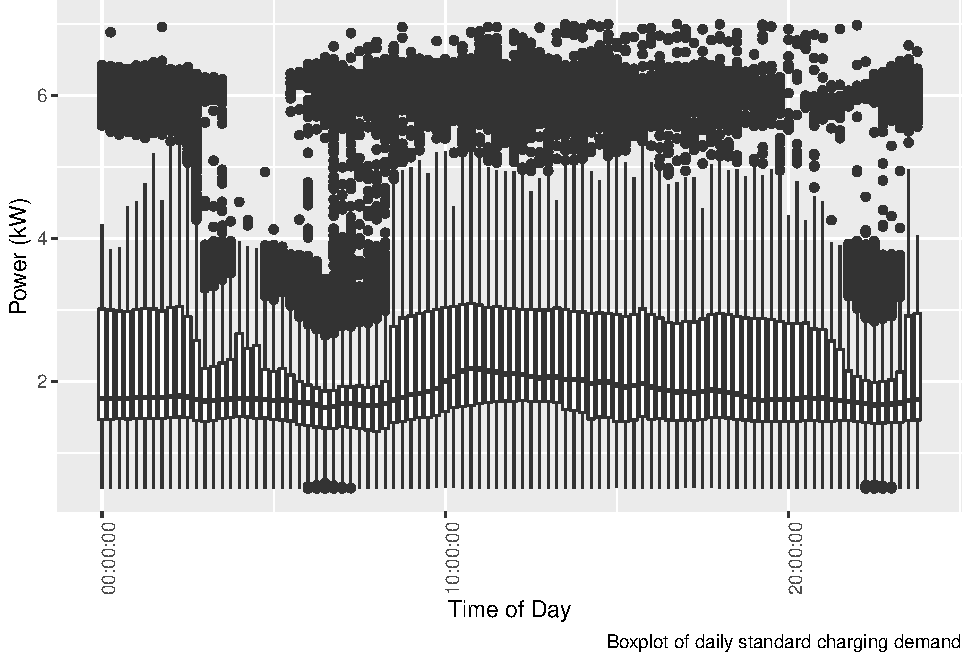
\includegraphics{EVBB_SummaryReport_files/figure-latex/boxplotCharging-1.pdf}
\caption{\label{fig:boxplotCharging}Boxplot of daily standard charging
demand}
\end{figure}

\begin{figure}
\centering
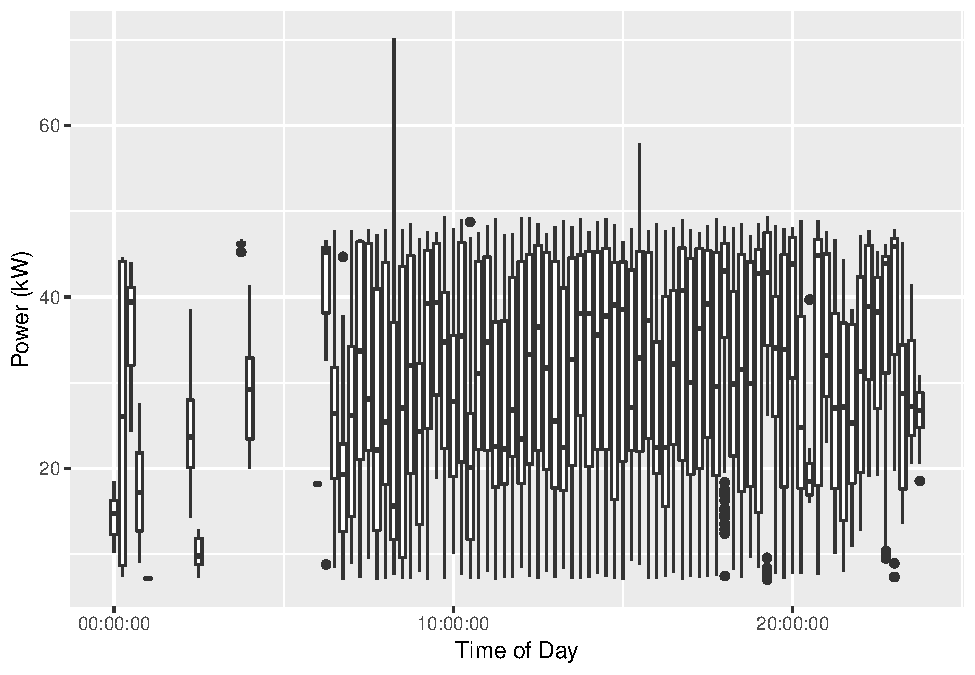
\includegraphics{EVBB_SummaryReport_files/figure-latex/plot3-1.pdf}
\caption{\label{fig:plot3}Boxplot of daily fast charging demand}
\end{figure}

\begin{verbatim}
## <ggproto object: Class FacetGrid, Facet, gg>
##     compute_layout: function
##     draw_back: function
##     draw_front: function
##     draw_labels: function
##     draw_panels: function
##     finish_data: function
##     init_scales: function
##     map_data: function
##     params: list
##     setup_data: function
##     setup_params: function
##     shrink: TRUE
##     train_scales: function
##     vars: function
##     super:  <ggproto object: Class FacetGrid, Facet, gg>
\end{verbatim}

\begin{figure}
\centering
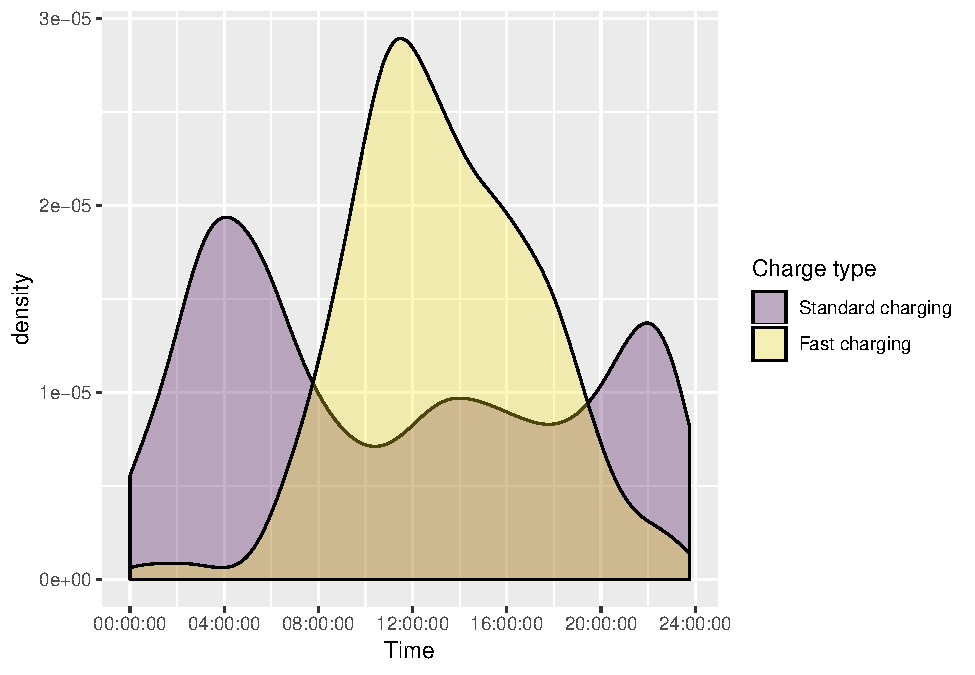
\includegraphics{EVBB_SummaryReport_files/figure-latex/chargeBeginsWeekday-1.pdf}
\caption{\label{fig:chargeBeginsWeekday}Density plot of charging start times
during weekdays}
\end{figure}

\begin{figure}
\centering
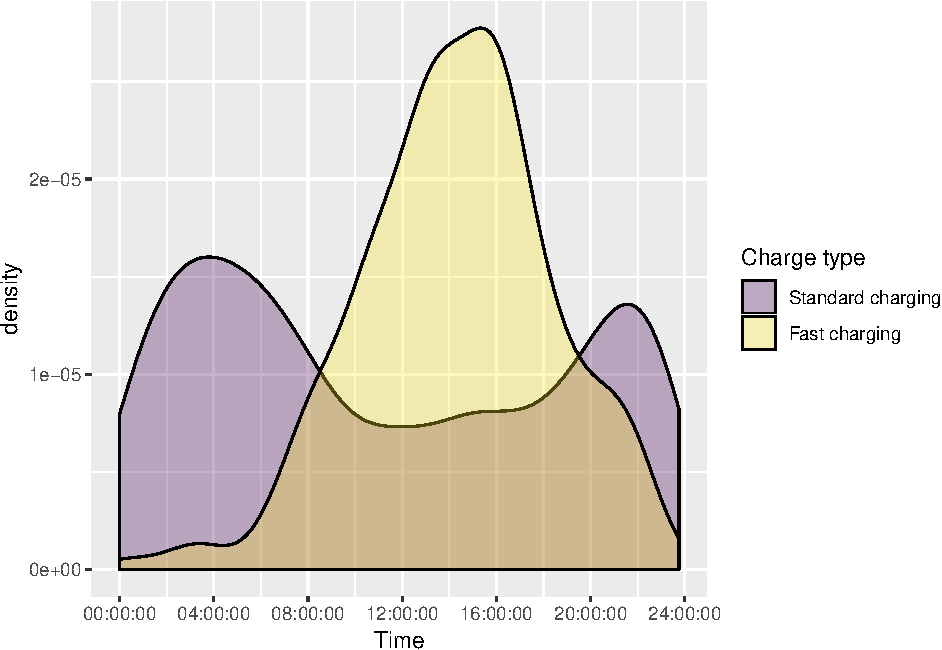
\includegraphics{EVBB_SummaryReport_files/figure-latex/chargeBeginsWeekend-1.pdf}
\caption{\label{fig:chargeBeginsWeekend}Density plot of charging start times
during weekends}
\end{figure}

\begin{figure}
\centering
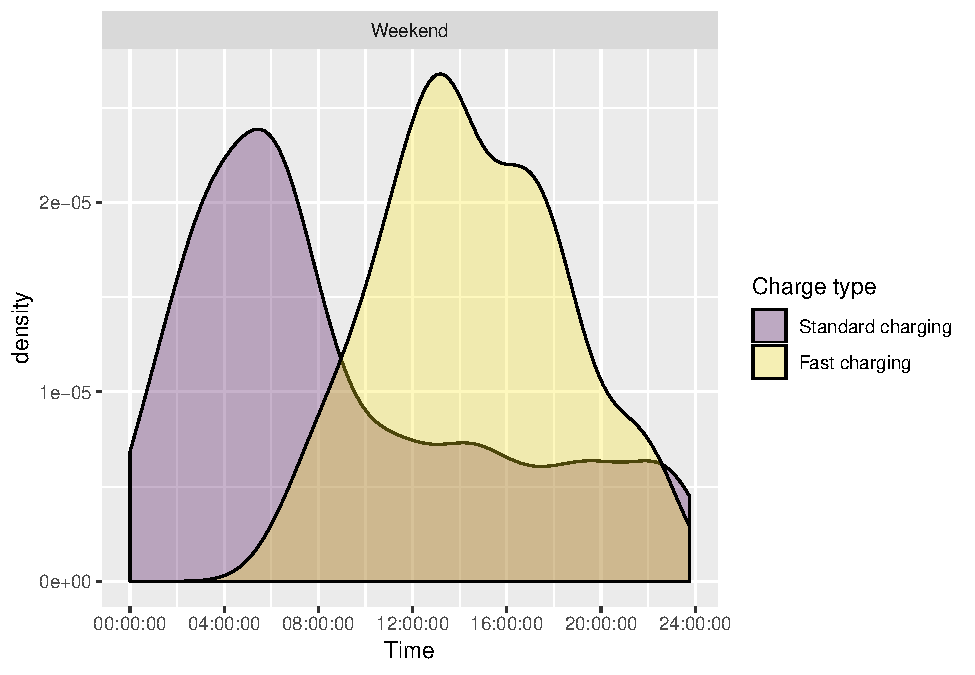
\includegraphics{EVBB_SummaryReport_files/figure-latex/chargeEndsWeekend-1.pdf}
\caption{\label{fig:chargeEndsWeekend}Density plot of charging end times
during weekends}
\end{figure}

Standard charging events tended to begin at HH:MM during weekdays and
HH:MM at weekends.

Standard charging has a noticeably different profile to charging
patterns for fast charges. It suggests that it is common for plug-in
vehicle owners to charge overnight at home, and perhaps use the more
powerful public chargepoints to top up during the day.

\begin{quote}
Discuss any other patterns
\end{quote}

\section{State of charge}\label{state-of-charge}

The duration of charging events (see Section \ref{duration}) suggests
that EVs may be `plugged in' at home (and elsewhere) for considerable
durations.

\begin{figure}
\centering
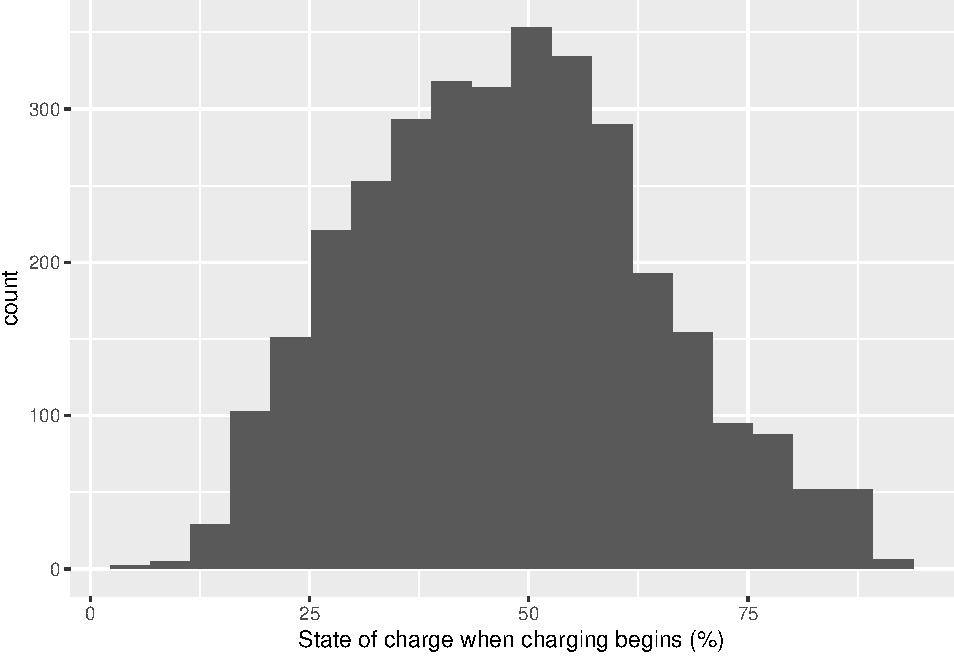
\includegraphics{EVBB_SummaryReport_files/figure-latex/SoCplot2-1.pdf}
\caption{\label{fig:SoCplot2}Value of state of charge at beginning of
charge}
\end{figure}

\begin{verbatim}
## Saving 6.5 x 4.5 in image
\end{verbatim}

Figure \ref{fig:SoCplot2} shows that many vehicles arrive home with
greater than 50\% charge remaining and would therefore be able to
transfer energy to the home during the evening grid peak as a form of
demand response.

Fig: Mean state of battery charge at the first `at home' charging
observation by hour and day of the week \emph{No ``at home'' data with
SOC}

\begin{quote}
should show the timing of `coming home' battery state?
\end{quote}

Fig: Distribution of duration of charge events starting `at home' in the
evening (by day of the week) \emph{Duration difficult to accurately
determine without date due to charging occurring through the night}

The figure shows that vehicles may then be available for further demand
response and/or re-charging for up to XX hours from this point.

\begin{quote}
Discuss any other patterns
\end{quote}


\end{document}
